% File: chapters/results.tex

\chapter{Experimental Results}
\label{chap:results}

Our three-phase research, conducted between May and September 2025 with infrastructure integration running in parallel with the initial local experiments, produced both expected and unexpected results. Some models generated working fuzz drivers while the majority did not. Fine-tuning improved efficiency but not coverage. Enterprise deployment was technically feasible but required more infrastructure work than anticipated. This chapter presents these findings in detail, organized by research phase, and maps them to the research questions from Chapter~1.


\section{Experimental Setup}
\label{sec:exp_setup}

\subsection{Target Selection and Criteria}
\label{sec:exp_targets}

Choosing appropriate target libraries required careful consideration. We needed C++ libraries because safety-critical automotive systems running on AUTOSAR (AUTomotive Open System ARchitecture) \cite{autosar} platforms are predominantly written in C or C++. AUTOSAR is the dominant software architecture standard for automotive electronic control units (ECUs), making C++ relevance essential for practical automotive application. While Python-based testing would have involved less complexity, C++ was selected to match the language used in safety-critical automotive systems at CARIAD.

After evaluating several candidates, we selected yaml-cpp as our primary target. This library parses YAML configuration files, a common task in automotive software where configuration management matters significantly. YAML is widely used in build systems, CI/CD pipelines, and deployment configurations across the automotive industry. The yaml-cpp library is found in several public repositories within automotive organizations including CARIAD. The library contains 35 source files with 1,061 potential fuzzing candidates identified through cifuzz spark analysis. It is also well-documented and actively maintained. OSS-Fuzz \cite{OSSFuzzBugs2021} already covers it, which provided a baseline for comparison. We could measure whether our AI-generated drivers matched, exceeded, or fell short of existing human-written ones.

Additional targets included pugixml, jsoncons, fmt, spdlog, and glm. These are widely used open-source C++ libraries that also appear in public repositories of automotive companies, including CARIAD's internal and public codebases. While they are not automotive-specific, they represent the types of general-purpose C++ dependencies commonly integrated into automotive software stacks for tasks such as XML/JSON configuration parsing (pugixml, jsoncons), log management (spdlog), string formatting (fmt), and mathematical computations for sensor processing (glm). These provided broader validation across different library types, and results for the top-performing models on these libraries are presented in Section~\ref{sec:results_cross_library}.


\subsection{Hardware and Software Configuration}
\label{sec:exp_hardware}

All local experiments ran on macOS with an Apple M1 Pro processor. The container runtime used Podman with 4 CPUs and 8 GB memory allocated. This choice was deliberate. We wanted hardware that typical automotive development teams have access to. If our approach required dedicated GPU clusters, practical adoption would be more constrained.

Our software stack consisted of Podman for containers (chosen to match the Linux-based container runtime used in the enterprise CI/CD environment), CMake with Clang for building, libFuzzer via cifuzz for fuzzing, and Ollama for local model inference. For enterprise deployment testing, we used Azure OpenAI with GPT-4o connected via Azure Private Link, a configuration established through the enterprise provisioning process, as detailed in Chapter~4.


\section{LLM Fuzz Driver Generation Results}
\label{sec:results_generation}

\subsection{Successful Models: Performance Data}
\label{sec:results_successful}

We evaluated models across different size categories on the yaml-cpp repository. The results, summarized in Table~\ref{tab:model_performance}, revealed several unexpected patterns.

\begin{table}[htbp]
\centering
\caption{Model Performance Metrics on yaml-cpp Repository}
\label{tab:model_performance}
\resizebox{\textwidth}{!}{%
\begin{tabular}{lccccc}
\toprule
Model & Code Coverage & Time Taken & Tokens Used & Unique Test Cases & Successful Tests \\
\midrule
Qwen 2.5-Coder 32B & 43.08\% & 32m 57s & 45.1k & 2,040 & 2 \\
Gemma 3 27B & 45.06\% & 33m 33s & 40.2k & 2,050 & 2 \\
Phi-4 14B & 34.26\% & 36m 36s & 71.5k & 2,220 & 1 \\
\bottomrule
\end{tabular}%
}
\end{table}

The ``Successful Tests'' column requires explanation, as this metric counts tests that discovered actual bugs or edge cases, not tests that simply compiled and ran. Most generated tests exercised valid code paths without finding vulnerabilities, which is expected behavior, not failure. The high number of unique test cases with few ``successful'' findings reflects that fuzzing is a volume-based process where many tests are generated with the expectation that a subset will discover issues. It is important to note that all three models listed in Table~\ref{tab:model_performance} produced drivers that compiled and ran successfully. The remaining eleven models (discussed in Section~\ref{sec:results_unsuccessful}) failed at the generation stage: their outputs either did not compile due to syntax errors, missing includes, or incorrect API usage, or crashed immediately at runtime due to invalid function calls. These models are therefore not included in Table~\ref{tab:model_performance} because they did not reach the fuzzing stage.

Line coverage measures the percentage of source code lines executed during testing. It is the standard metric we use throughout this thesis for evaluating fuzz driver quality (measured via \texttt{llvm-cov}). Gemma~3 27B achieved the highest coverage at 45.06\%, slightly outperforming the larger Qwen~2.5-Coder 32B, which reached 43.08\%. This was unexpected. The smaller model outperformed the larger one while using fewer tokens. We initially suspected measurement error, but the results held across multiple runs with consistent reproducibility.

That said, these numbers require context. While 45\% coverage represents a meaningful automated achievement, we examined several comparable manually-written fuzz drivers in the OSS-Fuzz corpus for yaml-cpp and similar parsing libraries (pugixml, RapidJSON, libxml2). These expert-crafted drivers typically achieve 60 to 80\% line coverage, based on coverage reports available through the OSS-Fuzz project dashboards\footnote{\url{https://introspector.oss-fuzz.com/}}. Our best AI-generated driver falls short of expert human work in absolute coverage terms. The value proposition is not matching expert coverage levels but automating fuzz driver creation, a task that would otherwise require considerable manual effort.

Phi-4 14B showed lower coverage at 34.26\% despite generating more unique test cases (2,220 vs 2,050). It required significantly more tokens, 71.5k compared to Gemma's 40.2k, making it considerably less efficient for production use. More test cases do not necessarily mean better coverage.

The comparative performance of these three successful models is visualized in Figure~\ref{fig:model_comparison}. Gemma 3 27B and Qwen 2.5-Coder 32B achieved the highest coverage levels (45\% and 43\% respectively), while Phi-4 14B reached 34\%. Only these three of the fourteen evaluated models produced functional fuzz drivers that reached the fuzzing stage. The remaining eleven models did not produce functional output at the code generation stage and are discussed in Section~\ref{sec:results_unsuccessful}.

\begin{figure}[htbp]
\centering
\caption{Code Coverage by Model (yaml-cpp). Only three of the fourteen evaluated models produced functional fuzz drivers.}
\label{fig:model_comparison}
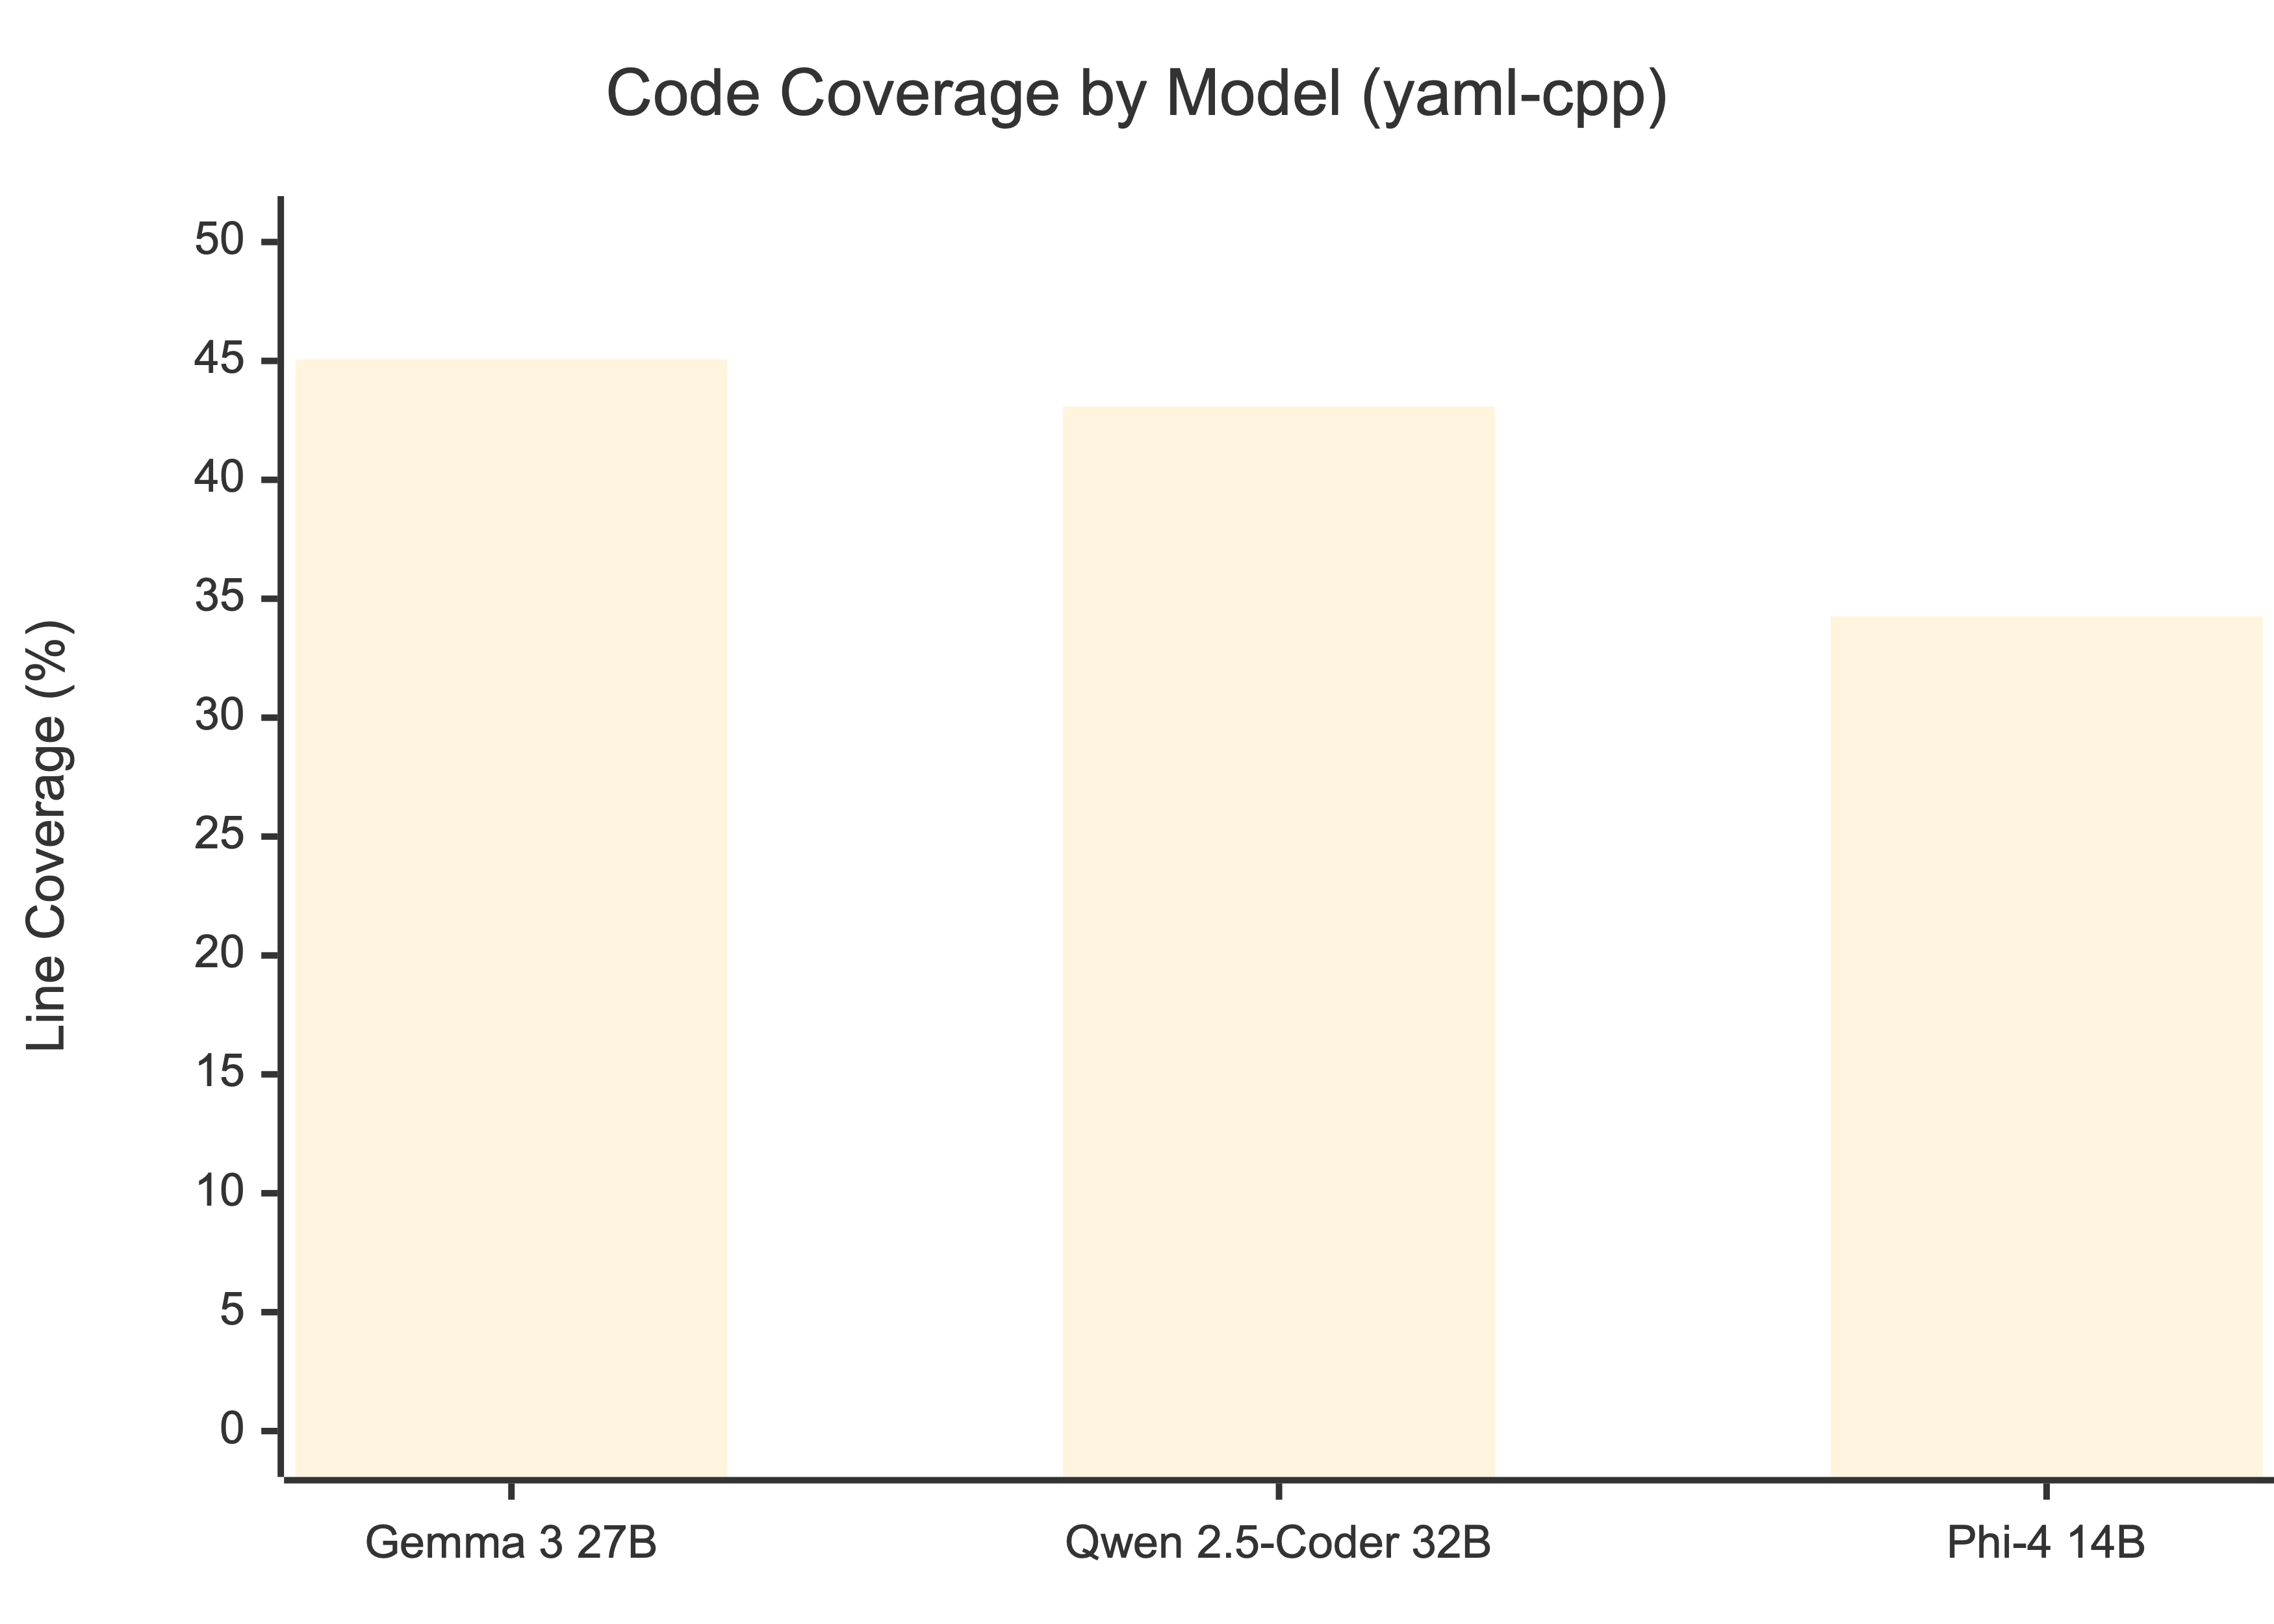
\includegraphics[width=\linewidth]{bilder/figure5_1_model_performance.png}
\end{figure}


\subsection{Unsuccessful Models: Critical Findings}
\label{sec:results_unsuccessful}

Several models did not produce usable output, as summarized in Table~\ref{tab:unsuccessful_models}. This was one of the more important findings of the research.

\begin{table}[htbp]
\centering
\caption{Unsuccessful Models and Failure Analysis on yaml-cpp}
\label{tab:unsuccessful_models}
\resizebox{\textwidth}{!}{%
\begin{tabular}{llll}
\toprule
Model & Parameters & Failure Stage & Failure Reason \\
\midrule
Qwen 2.5-Coder 14B & 14B & Compilation & Incorrect API usage, missing includes \\
Qwen 2.5-Coder 7B & 7B & Compilation & Incomplete driver structure \\
Qwen 2.5-Coder 1.5B & 1.5B & Compilation & Insufficient context understanding \\
DeepSeek Coder 33B & 33B & Compilation & Wrong function signatures \\
DeepSeek Coder V2 Lite & 16B & Compilation & Incomplete driver output \\
CodeLlama 34B Instruct & 34B & Compilation & Structural errors in generated code \\
WizardCoder 34B & 34B & Compilation & Malformed driver structure \\
Yi 34B & 34B & Runtime & Generation hallucinations, 0\% coverage \\
Gemma 3 9B & 9B & Compilation & Insufficient model capacity \\
Gemma 3 4B & 4B & Compilation & Insufficient model capacity \\
Mixtral 46.7B & 46.7B & Infrastructure & Model exceeded available hardware capacity \\
\bottomrule
\end{tabular}%
}
\end{table}

The majority of models failed at the compilation stage, producing code with syntax errors, incorrect API usage, or incomplete driver structures. Yi~34B was a notable exception: it produced code that compiled in some cases but achieved zero percent coverage at runtime. The generated drivers were syntactically valid but did not exercise the target library effectively. Functions were called with incorrect parameter combinations, or the driver simply returned immediately without exercising any library functionality. We tested variations of the prompt template to verify this was not a prompt engineering issue, and selected the version that most consistently produced compilable output. The results were consistent across attempts.

We also tested DeepSeek~R1, a reasoning-focused model, outside the original 14-model benchmark. It was designed for reasoning tasks, but in our experiments, that capability did not translate to effective fuzz driver generation. Mixtral's 46.7 billion parameters exceeded the available hardware capacity, preventing completion of a full evaluation run.

A clear pattern emerged from Table~\ref{tab:unsuccessful_models}. Code-specialized models outperformed larger general-purpose models by wide margins. Size alone does not determine quality for specialized tasks like fuzz driver generation. Furthermore, even among code-specialized models, only those with sufficient training on relevant code patterns (such as Qwen~2.5-Coder 32B) succeeded, while others (CodeLlama 34B, WizardCoder 34B) failed despite their code-focused training.


\subsection{Cross-Library Validation}
\label{sec:results_cross_library}

To validate whether the yaml-cpp findings generalize to other libraries, we tested the top-performing models on additional C++ targets. Not all models were evaluated on every library due to time constraints, so we focused on the models that showed the most promise.

\textbf{fmt (formatting library):}

Table~\ref{tab:fmt_results} presents the results for the fmt library. In addition to the 14 models from our primary benchmark, we tested Llama~3 and Qwen~1.5~7B on fmt to broaden coverage across model families.

\begin{table}[htbp]
\centering
\caption{Model Performance on fmt Library}
\label{tab:fmt_results}
\small
\begin{tabular}{lcccc}
\toprule
Model & Code Coverage & Time Taken & Tokens Used & Result \\
\midrule
Phi-4 14B & 100\% & 12m 8s & 59.8k & Successful \\
Llama~3 & 100\% & 3m 41s & 27.6k & Successful \\
Qwen~1.5 7B & 89.47\% & 6m 9s & 50k & Successful \\
Qwen 2.5-Coder 32B & 0\% & 43m 20s & 59.8k & Unsuccessful \\
Gemma 3 27B & 0\% & 41m 59s & 73.9k & Unsuccessful \\
\bottomrule
\end{tabular}
\end{table}

Table~\ref{tab:fmt_results} presents results that are counterintuitive compared to the findings from Section~\ref{sec:results_successful}. The two best-performing models on yaml-cpp (Qwen~2.5-Coder 32B and Gemma~3 27B) both achieved 0\% on fmt, while smaller models achieved near-perfect coverage.

We examined the generated outputs to understand this reversal. The fmt library exposes a small, well-documented API surface with clear input/output contracts (e.g., \texttt{fmt::format(format\_string, args...)}). The smaller models generated concise drivers that directly called these formatting functions with the fuzzer-provided input. In contrast, the larger models generated verbose, over-engineered drivers that attempted to construct complex formatting scenarios but introduced compilation errors or invalid API sequences in the process. Specifically, Qwen~2.5-Coder 32B generated drivers that referenced internal fmt implementation details not exposed in the public headers, while Gemma~3 27B produced drivers that called deprecated or non-existent overloads.

This observation is consistent with findings by Zhang et al.~\cite{LLMDriverGenEffectiveness2023}, who reported that LLM-generated fuzz drivers for simpler APIs achieve higher success rates, and that larger models do not uniformly outperform smaller ones across different target complexities. The key factor appears to be the match between model output verbosity and API complexity: simpler APIs benefit from concise, targeted generation, while complex APIs like yaml-cpp require the broader context understanding that larger models provide. This finding reinforces that no single model dominates across all library types, and model selection should consider the target API characteristics.

\textbf{pugixml (XML processing library):}

The results for fuzz-testing code from the pugixml library are presented in Table~\ref{tab:pugixml_results}.

\begin{table}[htbp]
\centering
\caption{Model Performance on pugixml Library}
\label{tab:pugixml_results}
\small
\begin{tabular}{lcccc}
\toprule
Model & Code Coverage & Time Taken & Tokens Used & Result \\
\midrule
Qwen 2.5-Coder 32B & 34.77\% & 37m 24s & 43.1k & Successful \\
Gemma 3 27B & 0\% & 1h 12m 8s & 122k & Unsuccessful \\
\bottomrule
\end{tabular}
\end{table}

On pugixml, Qwen 2.5-Coder 32B achieved 34.77\% coverage, comparable to its yaml-cpp performance (43.08\%). Gemma 3 27B did not achieve any coverage despite consuming considerably more tokens (122k vs 40.2k on yaml-cpp), suggesting the XML parsing API posed challenges that the model was not able to address in this configuration.

\textbf{jsoncons, glm, and spdlog (Qwen 2.5-Coder 32B only):}

Table~\ref{tab:additional_libraries} summarizes the results for testing jsoncons, glm, and spdlog.

\begin{table}[htbp]
\centering
\caption{Qwen 2.5-Coder 32B Performance Across Additional Libraries}
\label{tab:additional_libraries}
\resizebox{\textwidth}{!}{%
\begin{tabular}{lccccc}
\toprule
Library & Code Coverage & Time Taken & Tokens Used & Test Cases & Successful Tests \\
\midrule
jsoncons & 45.64\% & 37m 24s & 43.1k & 2,500 & 1 \\
glm & 0\% & 42m 55s & 56.8k & 0 & 0 \\
spdlog & 0\% & 49m 33s & 62.9k & 0 & 0 \\
\bottomrule
\end{tabular}%
}
\end{table}

As shown in Table~\ref{tab:additional_libraries}, jsoncons showed the highest coverage of any library we tested (45.64\%), slightly exceeding even yaml-cpp. Both are parsing libraries with similar API patterns, which may explain the consistency. glm (a mathematics library for graphics) and spdlog (a logging library) both produced 0\% coverage, indicating that the models did not generate effective drivers for non-parsing API patterns. Libraries with mathematical or configuration-heavy interfaces appear more challenging for current LLMs.

\textbf{Cross-library summary:} The results show that model performance varies considerably across libraries. Parsing libraries (yaml-cpp, jsoncons, pugixml) consistently produced the highest coverage, while utility libraries (glm, spdlog) were more challenging. Library complexity did not always predict difficulty, as fmt's simpler API yielded perfect coverage with smaller models. These findings suggest that API style and documentation quality matter more than library size or domain.


\section{Model Optimization Results}
\label{sec:results_optimization}

Having established that specialized models outperform general-purpose ones, we investigated whether fine-tuning could further improve efficiency while reducing computational requirements. These experiments address the optimization aspect of \textbf{RQ2}: can smaller models with domain-specific training match or exceed larger general-purpose models?

\subsection{LoRA Fine-Tuning Efficiency}
\label{sec:results_lora_efficiency}

Based on Phase 1 results, we selected the Qwen 2.5-Coder 1.5B model for fine-tuning experiments. The goal was to determine whether a small, fine-tuned model could match larger models while using markedly fewer resources.

We applied Low-Rank Adaptation (LoRA) \cite{Hu2021} fine-tuning using fuzz drivers from Google's OSS-Fuzz project as training data. LoRA works by freezing most of the original model weights and inserting small trainable matrices into the attention layers, so only a fraction of parameters are updated during training. This makes fine-tuning feasible on consumer hardware without the memory requirements of full model training. Our approach builds on recent work in LLM-based fuzzing \cite{llm4fuzz,TitanFuzz2022} but applies more aggressive model compression through fine-tuning. We curated two training datasets from publicly available OSS-Fuzz repositories, a small one with 172 examples and an extended one with 709 examples. Each example consisted of a fuzz driver paired with its target API context, covering security vulnerability patterns, fuzzing techniques, and automotive-specific code patterns.

Our fine-tuning configuration:
\begin{itemize}
    \item LoRA Rank: 16
    \item LoRA Alpha: 32
    \item Dropout: 0.1
    \item Target Modules: q\_proj, v\_proj, k\_proj, o\_proj
    \item Precision: float16
\end{itemize}

Results showed measurable efficiency improvements:

\begin{table}[htbp]
\centering
\caption{LoRA Fine-Tuning Efficiency Improvements}
\label{tab:lora_efficiency}
\small
\begin{tabular}{lccc}
\toprule
Model Version & Time Taken & Tokens Used & Efficiency Improvement \\
\midrule
Base 1.5B & 15 min & 112k & Baseline \\
172 examples & 12 min & 65k & 20\% faster, 42\% fewer tokens \\
709 examples & 10 min & 50k & 33\% faster, 55\% fewer tokens \\
\bottomrule
\end{tabular}
\end{table}

With 709 examples, the extended dataset produced the largest improvements with 33\% faster generation and 55\% fewer tokens compared to the base model. The fine-tuned model learned to generate more concise, targeted code rather than verbose outputs padded with unnecessary boilerplate.


\subsection{Comparative Analysis}
\label{sec:results_lora_analysis}

Training data quality and quantity both matter, though quality appears more important. The 709-example dataset outperformed the 172-example dataset, but the improvement was incremental rather than dramatic. More diverse examples help the model generalize, but there are diminishing returns.

One key insight is that a fine-tuned small model can match larger models while using markedly fewer computational resources. This makes enterprise deployment practical, as it does not require expensive GPU infrastructure to run effective fuzz driver generation.

However, we should note the limitations. The fine-tuned 1.5B model still does not match the coverage achieved by the larger Qwen 32B or Gemma 27B models. What it offers is efficiency, acceptable coverage at much lower cost and resource requirements.

The efficiency gains from fine-tuning directly impact deployment feasibility in resource-constrained environments. However, efficiency alone does not determine practical viability, cost considerations also play a major role in enterprise adoption.


\section{Economic Analysis and Resource Metrics}
\label{sec:results_economics}

Beyond technical performance, successful enterprise deployment requires favorable economics. This section addresses the cost component of \textbf{RQ3}: Can LLM-assisted fuzz driver generation be integrated into secure enterprise CI/CD pipelines while meeting performance, cost, and security requirements? As defined in Chapter~4 (Section~\ref{sec:impl_phase3}), the performance requirements include completing driver generation within the 15 to 30 minute CI/CD feedback window, the cost requirements cap annual infrastructure spending below \euro{}2,000, and the security requirements mandate that no proprietary source code leaves the corporate network. We analyzed both direct infrastructure costs and opportunity costs relative to manual approaches.

We analyzed costs in detail because the question is not only ``does this work?'' but ``is this economically viable for real deployment?''

\subsection{Azure OpenAI Cost Projections}
\label{sec:results_cost_azure}

Based on Azure OpenAI pricing as of July 2025 (the time of our experiments):

\begin{table}[htbp]
\centering
\caption{Azure OpenAI Cost Projections for Different Usage Levels}
\label{tab:cost_scenarios}
\small
\begin{tabular}{lcccc}
\toprule
Usage Level & Daily Cost & Monthly Cost & Annual Cost & Use Case \\
\midrule
Light & \euro{}0.28 & \euro{}6.16 & \euro{}73.92 & Development/testing \\
Moderate & \euro{}0.83 & \euro{}18.26 & \euro{}219.12 & Small team production \\
Heavy & \euro{}2.75 & \euro{}60.50 & \euro{}726.00 & Full enterprise deployment \\
Enterprise & \euro{}5.50 & \euro{}121.00 & \euro{}1,452.00 & Complete automation \\
\bottomrule
\end{tabular}
\end{table}

Even at the enterprise level with complete automation, annual costs stay under \euro{}1,500. This is minimal compared to manual security testing approaches. However, this represents only the direct infrastructure costs.


\subsection{Comparison with Manual Testing}
\label{sec:results_cost_manual}

Industry estimates for manual fuzz driver development:
\begin{itemize}
    \item Senior security engineer hourly rate: \euro{}80 to 120 (based on published industry benchmarks)
    \item Time to write an effective fuzz driver: 2 to 8 hours per target (lower end for well-documented parsing APIs, upper end for complex C++ libraries with heavy template usage)
    \item Annual cost for security engineering resources: varies by market and seniority
\end{itemize}

The AI-driven approach offers:
\begin{itemize}
    \item Infrastructure cost: \euro{}219-\euro{}1,452 annually
    \item Estimated time savings: 75 to 94\% reduction in initial driver creation time (based on comparison of approximately 30 minutes automated generation vs. 2 to 8 hours of manual writing per target)
\end{itemize}

The economic advantage appears clear, but there is an important caveat. Current LLMs do not incorporate domain-specific automotive safety requirements, do not account for ISO 26262 compliance considerations, and may occasionally generate tests that are syntactically correct but lack semantic depth. It should be noted that none of the test cases in our evaluation incorporated safety-related constraints (e.g., ASIL levels, timing requirements, or fault-tolerance checks); all generated drivers focused exclusively on functional correctness and coverage of the public API surface. Human oversight remains essential. The time savings estimate assumes engineers spend their time reviewing and improving AI-generated drivers rather than writing from scratch, not that AI fully replaces human judgment. The cost of this human oversight is not captured in the infrastructure costs above, and the actual savings will vary depending on the complexity of the target library and the quality of the generated driver.


\section{Summary}
\label{sec:results_summary}

The experiments produced several clear findings, along with some important caveats.

Model specialization matters more than size. Gemma 3 27B outperformed Yi 34B despite having fewer parameters. Code-specialized models outperformed larger general-purpose models consistently across our tests.

Performance also varies across library types. Parsing libraries (yaml-cpp, jsoncons, pugixml) consistently produced the best coverage results, while utility libraries (glm, spdlog) proved more challenging. The fmt library revealed that smaller models can outperform larger ones on simpler APIs, with Phi-4 14B and Llama~3 achieving 100\% coverage where the larger Qwen~2.5-Coder 32B and Gemma~3 27B both achieved 0\%.

Fine-tuning enables efficient deployment. The fine-tuned 1.5B model achieved 33\% faster generation and 55\% fewer tokens compared to the base model, though it still did not match the coverage of larger specialized models.

The economics appear favorable as well. Annual infrastructure costs range from \euro{}74 for light usage to \euro{}1,452 for full enterprise deployment. Manual security engineering involves higher personnel investment, though the two approaches serve complementary rather than interchangeable functions. The LLM automates initial driver creation while human expertise remains necessary for review and refinement.

Mapping these findings to our research questions:

\textbf{RQ1 (Effectiveness)}: Can Large Language Models generate fuzz drivers for C++ code that compile successfully, execute without errors, and achieve meaningful code coverage? The results support this at least to some extent. Our best models achieved over 40\% coverage on yaml-cpp and up to 100\% on fmt, with drivers that compiled and executed correctly. Cross-library testing (Section~\ref{sec:results_cross_library}) confirmed these results generalize to other parsing libraries like jsoncons (45.64\%) and pugixml (34.77\%), though performance on non-parsing libraries was more variable. We consider 34 to 45\% coverage ``meaningful'' because it represents automated baseline coverage that would otherwise require 2 to 8 hours of manual engineering per target. While this falls short of expert human-written drivers (60 to 80\% coverage), the value lies in automation at scale, not matching human experts.

\textbf{RQ2 (Optimization)}: Does model size determine fuzz driver quality, or can smaller models with domain-specific training match or exceed larger general-purpose models? Smaller specialized models consistently outperformed larger general-purpose models. Fine-tuning further improved efficiency, though not coverage.

\textbf{RQ3 (Feasibility)}: Can LLM-assisted fuzz driver generation be integrated into secure enterprise CI/CD pipelines while meeting performance, cost, and security requirements? Integration proved feasible at costs under \euro{}1,500 annually, but the process required careful infrastructure planning (Azure Private Link) to meet the security requirements of regulated environments.